In our system design, two types of dataset are needed. The first is the social media textual data, which is the most vital to this system, called social media dataset. It contains the implication of potential outbreak of diseases or other healthcare-related information, all the prediction will be made based on it. In addition, to evaluate the model convincingly, actual records of diseases and additional labeled data are needed to serve as benchmark. 
\section{Social media dataset}
\label{sec:Social media dataset}
Researchers have used the Web as sources of syndromic surveillance for years, including Google Flu Trends (display the statistics of daily query logs related to influenza), Twitter, Facebook \cite{paul2011you}. 
In this project, we choose one certain social media platform to test our algorithm, that is Twitter. More specifically, we focus on tweets expressed in English. These choices based on the characteristics of Twitter:
\begin{itemize}
    \item Providing location: In our design, the posting location of each post is required. And we found that Twitter provides such information. According to research conducted by \cite{greenwood2016social} in 2016, about 1.6 percent of Twitter users opted in Twitter's location-sharing service.
    \item Availability: Most tweets are available for research. According to \cite{serban2019real}, around 95\% of Twitter users opted in sharing their tweets with public, meaning their tweets can be searched and filtered by keywords without their permission.  
    \item Comparability: In our research, we found that most related works used data from Twitter, which means that Twitter dataset can act as a benchmark to evaluate our algorithm.
    \item Timely: According to \cite{serban2019real}, each tweet is received within seconds of their creation.
    \item High user volume: According to \cite{greenwood2016social}, about 21\% of American citizens use Twitter.
\end{itemize} 

\section{Benchmark}
For this project, the evaluation are conducted from multiple aspects: (1) whether a new document can be correctly identified as health-related or not; (2) whether the filtered documents can be properly grouped and get interpretable topics (including find new health event); (3) whether the trend shown in social media follows the actual diagnostic recording. First one aims to evaluate the performance our model, therefore, reliable healthcare-related tweets are required. The benchmark dataset is from the official Twitter account (such as CDCHealth, BBCHealth) and health-related Hashtags. To evaluate the criterion, labeled data are required, but they are not necessary to be health-related. The third one can help to verify the trustability and informativity of social media, real disease data are required. Centers for Disease Control and Prevention (CDC)\cite{cdc.gov} is a well-known nation's health protection agency recording diseases (such as flu, heart diseases, COVID-2019) and conditions over the US. Data published by CDC are comparably reliable. In this project, we focus on one disease, flu. The benchmark used in this project is Fluview \cite{cdc:fluView}, a weekly-update, influenza surveillance report of the U.S. published by CDC. Such report is a collaborative effort between CDC and its many partners in state, local, and territorial health departments, public health and clinical laboratories, vital statistics offices, healthcare providers, clinics, and emergency departments \cite{cdc.gov}. CDC maintains a surveillance network called Influenza-like Illness Surveillance Network (ILINet), which collect information on outpatient visits to health care providers for influenza-like illness \cite{cdc.gov}. We choose CDC's Fluview as our benchmark because of its:
\begin{itemize}
    \item Reliability: ILINet collects data from about 2600 outpatient healthcare providers across the U.S. weekly \cite{cdc.gov}.
    \item Accessibility: All the reports of Influenza-like Illness (ILI) can be accessed by public.
    \item Comparability: The dataset maps the activity of ILI into levels between 1 to 10, which can be used as labels or targets of our training data.
\end{itemize}
\begin{figure}[!htbp]
   \center
   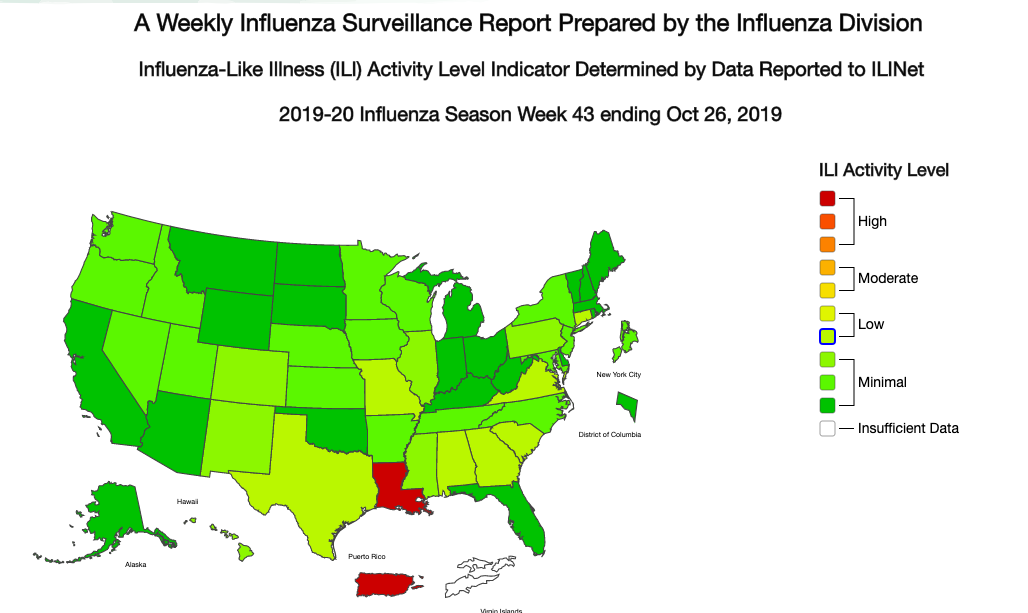
\includegraphics[width=6in]{images/week43.png}
   \caption{Influenza Season Week 43 ending Oct 26, 2019, Source: \href{https://www.cdc.gov/flu/weekly/index.htm\#ILIActivityMap}{Fluview}}
   \label{fig:fluView}
\end{figure}
Figure\ref{fig:fluView} shows the ILI activity levels across the U.S. in Week 43, 2019. It can be seen that the there are 10 levels divided into 3 categories, each level is assigned a unique color.

\section{Data collection}
\label{sec:Data collection}
This section shows the detailed methods of how we collect data and unify the data structure. 
\subsection{Twitter dataset collection}
\label{sec:Twitter dataset}
In this project, we collect Twitter data from Internet Archive\cite{archive}, a non-profit digital library of millions of free books, movies, software, music, websites. It contains daily tweets from Feb 2011 to Jul 2019 (Accessed: Dec 08,2019). All the data are Spritzer version (roughly 1\% of the whole tweets) grabbed from the general twitter stream The number of tweets collected in Oct 05 2018 is 4273031, in Oct 04 2018 is 4337327, in Oct 01 2018 is 4317376, on average is above 4 million per day. All the tweets are stored in json files. Such data volume is sufficient for our research and its data structure is convenient to use. More important, it contains the information we need, which mentioned in section \ref{sec:Social media dataset}. Figure \ref{fig:archive1} shows part of the information those json files contain (geographic and linguistic information are contained but not listed here). In our project, we mainly focus on tweets posted during 2018.\\
\begin{figure}[!htbp]
    \center
    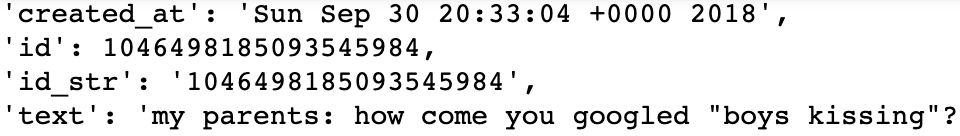
\includegraphics[width=5.5in]{images/archive1.png}
    \caption{Screenshot of Archive's Twitter data}
    \label{fig:archive1}
\end{figure} 

\subsection{Benchmark dataset collection}
\href{https://www.trackmyhashtag.com/blog/twitter-datasets-free/}{trackmyhashtag} (Accessed: March 25, 2020) provides more than 60K free tweets with hashtags ``COVID-19'' from 1st Dec, 2019 to 28 Jan 2020, and historical tweets posted by 16 official health-news Twitter accounts from 2012 to 2015. Those data can be treated as real healthcare-related tweets and they are used to evaluate the supervised model in our design. \cite{qiang2018STTP} published 6 labeled short text datasets for unsupervised clustering algorithm on \href{https://github.com/qiang2100/STTM}{their GitHub} (Accessed: March 25, 2020). We use part of them to evaluate our unsupervised model. Fluview data can be downloaded from official websites of CDC \cite{cdc:fluView} (Accessed: Dec 08,2019), user can customize the data they want to download (the time span of reports). 

\section{Data Preprocessing}
\label{sec:Preprocessing}
Data preprocessing is the first stage of a typical text classification framework. According to experiment conducted by \cite{uysal2014impact}, different combination of preprocessing methods can influence the accuracy of prediction. However, there is no best combination for all tasks. Some strategies can improve classification success of certain tasks while lower that of others.
\begin{figure}[!htbp]
    \centering
    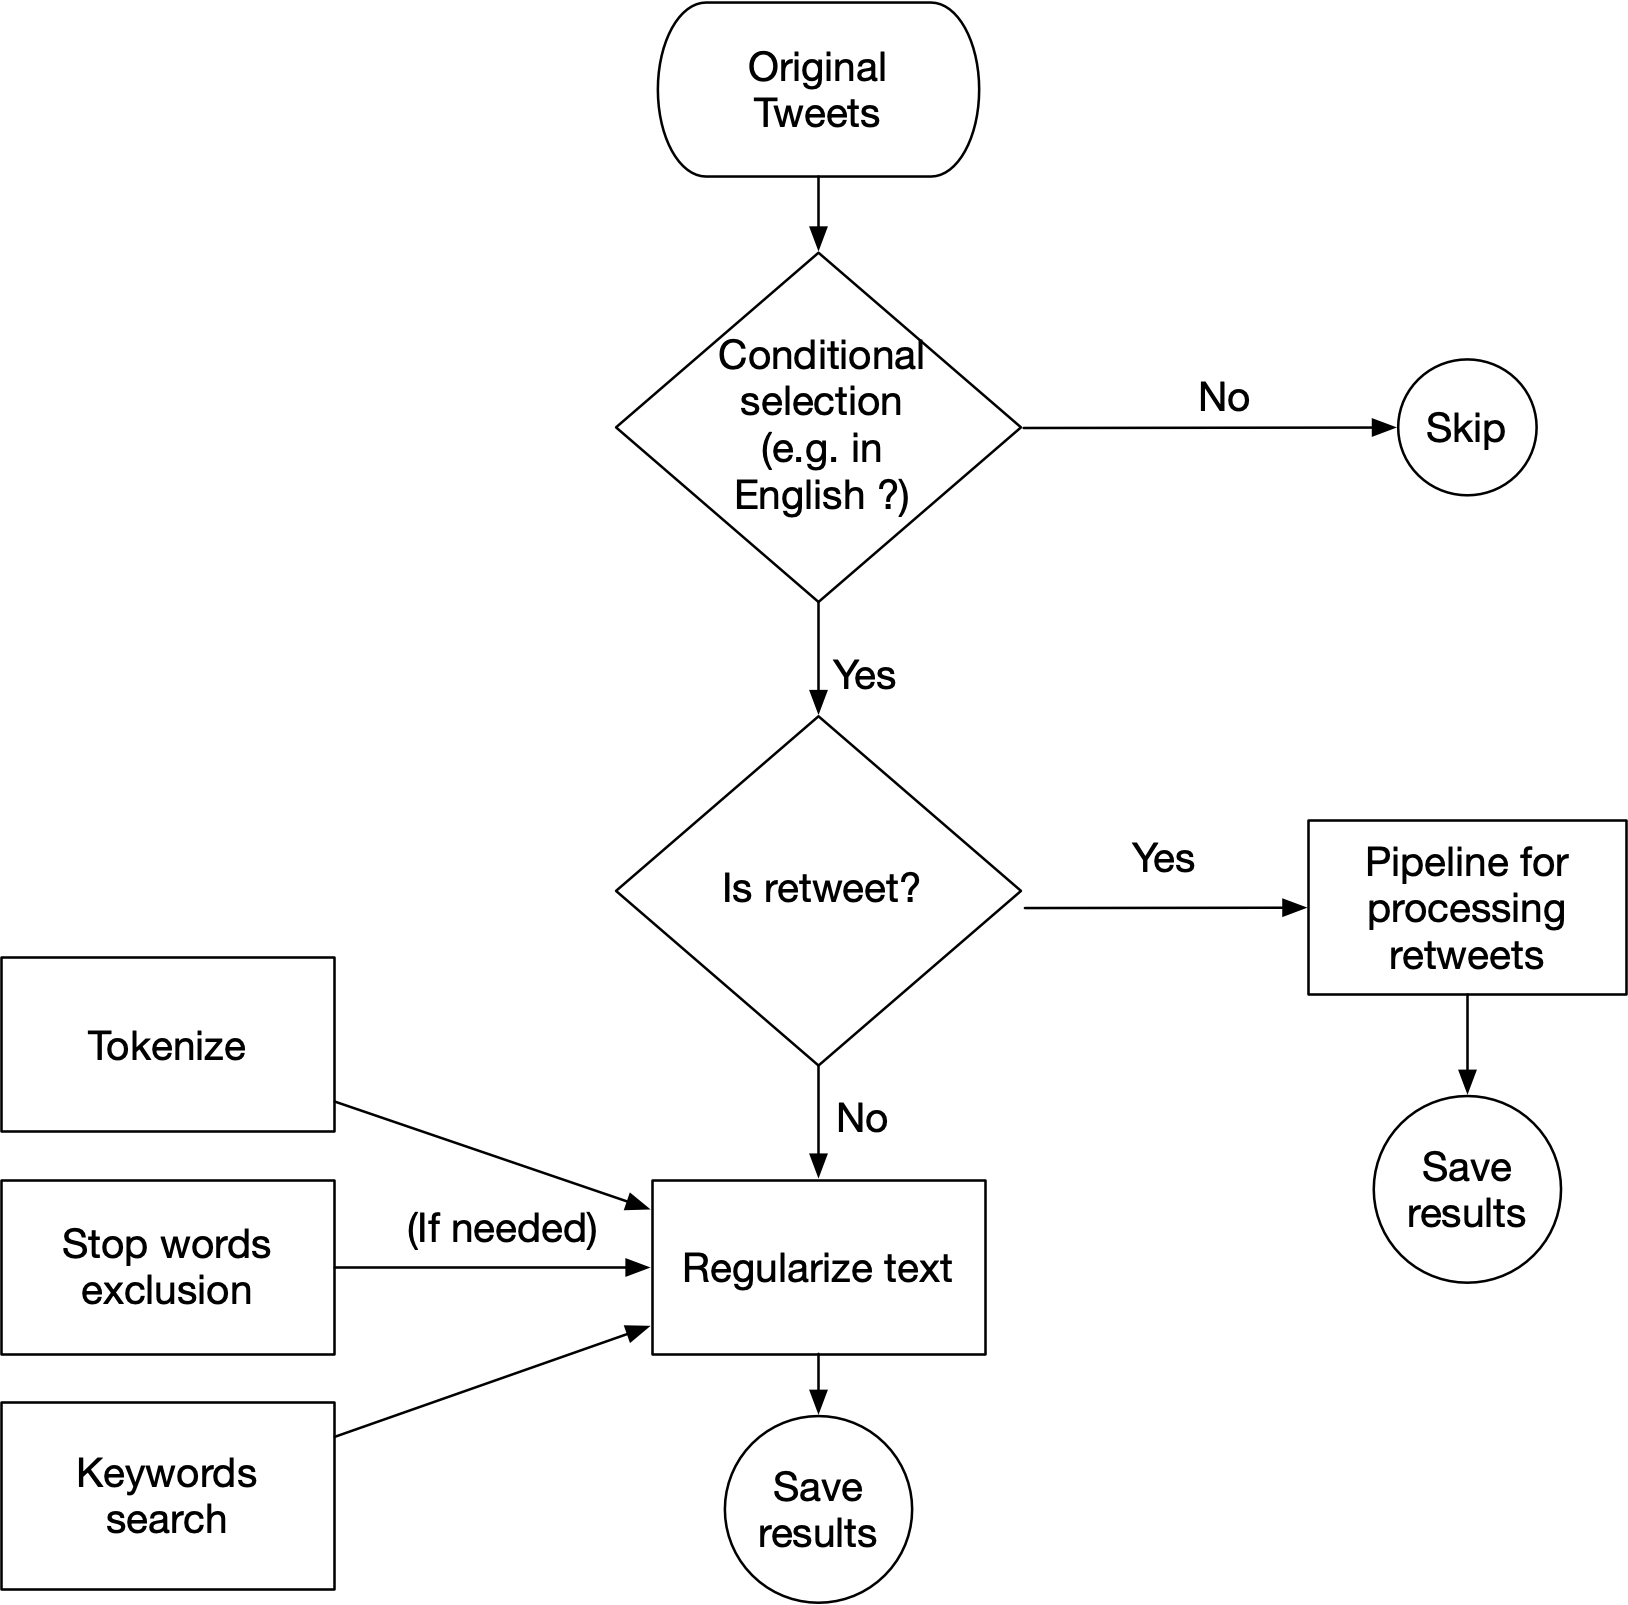
\includegraphics[height=3in]{pipeline.jpg}
    \caption{Common pipeline of text preprocessing}
    \label{fig:pipeline}
\end{figure} 
Figure \ref{fig:pipeline} shows some common steps used in NLP for preprocessing textual data. Following sub-sections explain the details of our preprocessing methods designed for this project.
\subsection{Unify data structure}
\label{sec:Unify data structure}
In section \ref{sec:Data collector design}, we mentioned a unified data structure of our datasets. The aim of this stage is to unify and regularize all the metadata before analysis. \\
\\The Fluview dataset is well structured (see Figure \ref{fig:fluView1}), and can be used in our system directly (we used its ``STATENAME", ``ACTIVITY LEVEL", ``ACTIVITY LEVEL LABEL'' and ``WEEK'' columns). One point should be noticed here is that the STATENAME used in Fluview dataset can be different from that in Twitter (Twitter' users can set their own location), therefore, we created a unified name list of states and a function designed to regularize different geographic information.\\
\\
Our social media dataset's structure is built on Twitter's official data structure \cite{twitter_dev}, and we only retain the information we may use. It is a hashmap with 6 keys: ``created\_at'', ``text'', ``location'' and ``coordinates'', ``place'', ``hashtags''. We regularize the time into format Year/Month/Day (2018/10/01) and store it in ``created\_at'' keys, exclude other information. Note that in the metadata, there are massive ``deleted'' tweets, which contain no textual information, and we removed all such data. ``hashtags'' is not a original key in metadata. Hashtags are wildly used in social media and it explicitly indicate topics of tweets. With them, modeling and evaluation could be more accurate. 
\begin{figure}[!bp]
    \centering
    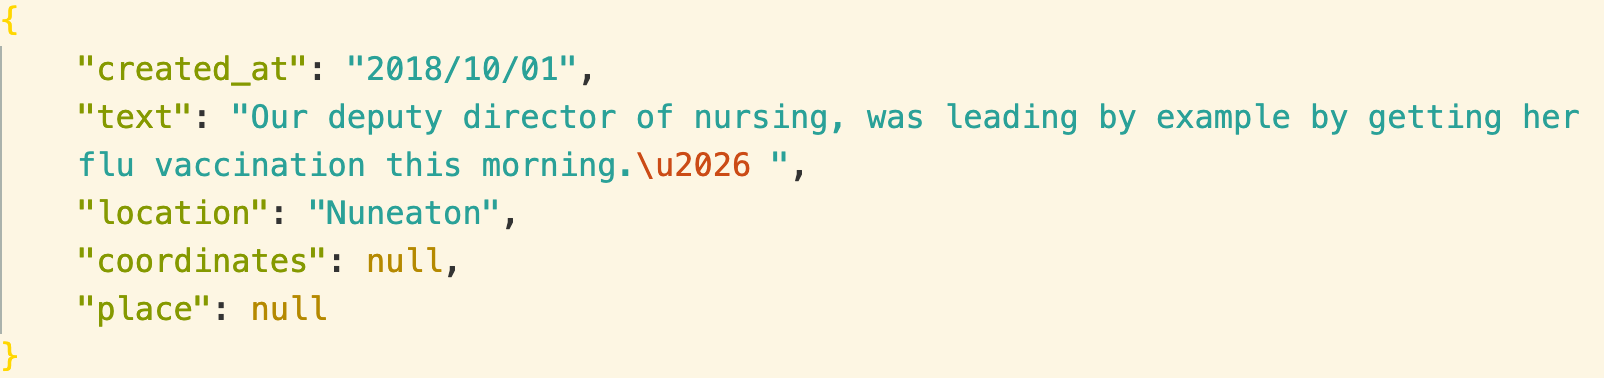
\includegraphics[width=5in]{images/dataset1.png}
    \caption{Screenshot of unified structure of social media dataset}
    \label{fig:social_data_sture}
\end{figure}
According twitter's official document \cite{twitter_dev}, there are two classes of geographical metadata in Tweet data: (1) Tweet location, which is available when users share location at time of Tweet; (2) Account Location: a free-form character field set in user's profile and may or may not contain metadata that can be geo-referenced. ``location'' attribute stores the user-defined placename. ``coordinates'' attribute provides the exact location of a tweet (in long-lat order) but has no placename and only available when the location is assigned. ``place'' attribute is always present when a Tweet is geo-tagged, and it contains Twitter ``place'' with a display name and type. Here we keep all these three keys, and ``place'' key gets the first priority when we extract location of tweet. Figure \ref{fig:twitter_place} shows a sample of Twitter ``place''. Note that most data don't contain ``location'', ``coordinates'' and ``place'' keys, which is expected in section \ref{sec:Social media dataset}.
\begin{figure}[!htbp]
    \centering
    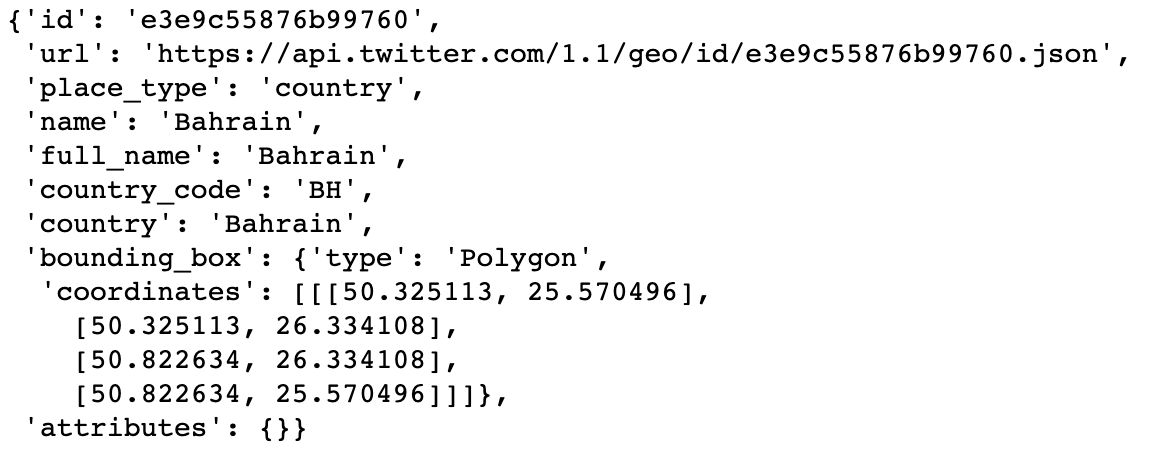
\includegraphics[width=5in]{images/twitter_place.png}
    \caption{Screenshot of Twitter's place object from our dataset}
    \label{fig:twitter_place}
\end{figure}

\subsection{Text regularization}
As mentioned in our design (\ref{sec:Data preprocessor design}), the original text is unstructured, which can not be put in to our model directly and hard for labeling. In addition, each dataset has its own structure, meaning that there is no common regularization rule can be applied to all tasks. Here our regularization rule is built on the observation of our dataset and on our judgement. Followings are common formats we observed in our dataset, expressed in regular expression (Python version):
    \begin{itemize}
        \item retweet: retweeting is a way of forwarding content to others (like forwarding an email). It starts with a ``RT \@'' pattern. 
        \item @: in social media, @ refers to a person/group in a conversation and has no meaning for analysis. Its regular expression is ``\@+[\verb|\|S]*''. 
        \item URL links: some tweets contain URL links starting with ``http'', ``ftp'' or ``https'', which can't contribute to our classification. Its regular expression is:\\``http[s]?://(?:[a-zA-Z]$|$[0-9]$|$[\$-\_@.\&+]$|$[!*\verb|\|(\verb|\|),]$|$(?:\%[0-9a-fA-F][0-9a-fA-F]))+''
        \item emoji: emojis in our dataset are encoded in unicode, inspired by \cite{serban2019real}, some of them can be translated into their name based on emoticon dictionaries. Through our search, we find a Python library called \href{https://pypi.org/project/emoji/} {emoji(version 0.5.4}), which embedded the full emoji list from \cite{emo_list} and can help us to translate emoji into text through function call \cite{pytho_emo}. Figue \ref{fig:emo_lib} shows a example how to use this library, the translated emojis are embraced by `:' signs by default. In our implementation, each translated emoji is assigned a prefix `emo\_' to identify it, and we separate emojis with a blank space for split convenience.
        \begin{figure}[!htbp]
            \centering
            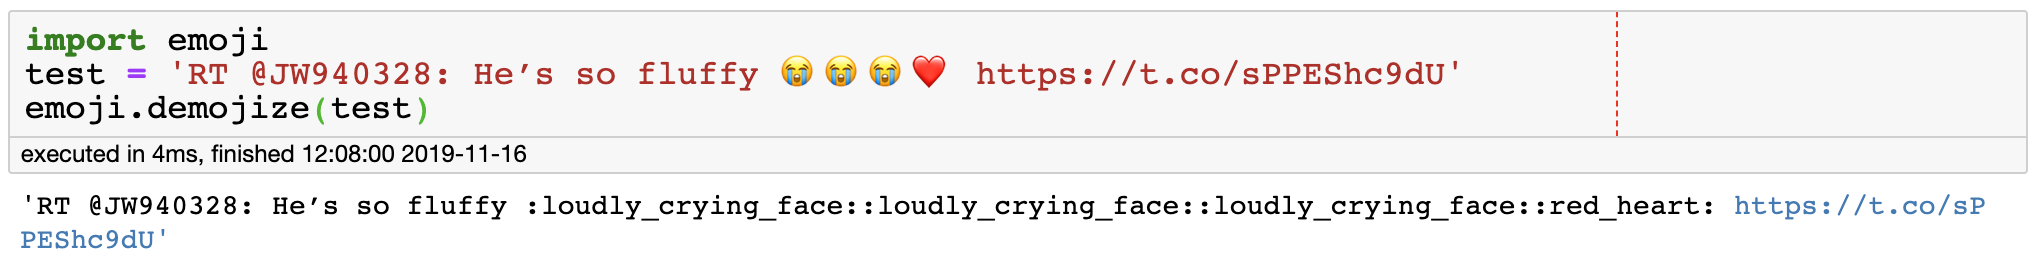
\includegraphics[width=5in]{images/emoji_lib.png}
            \caption{Example of using emoji library}
            \label{fig:emo_lib}
        \end{figure}
        \item e-mail address: we exclude e-mail address in our data, whose regex(can match most e-mail addresses) is:
        ``[a-zA-Z0-9\_.+-]+\@[a-zA-Z0-9-]+\verb|\|.[a-zA-Z0-9-.]+\$''
        \item html entities: a html entity can be regarded as escape characters used in html (eg. \&quot; represents ``'' sign). We use the Python's standard library ``html'' to translate it.
        \item non-Latin characters: characters that are not in Latin are meaningless, we exclude them with regex ``[\^A-Za-z0-9]'' 
        \item hashtags \#: In social media, hashtags explicitly indicate topics of documents. Its regex can be written as ``[\#]{1}(\\w+)''
    \end{itemize}
For convenience, all characters of processed documents are in lower case. 

\subsection{Manually screening}
\label{sec:Manually screening}
We have more than 4 million tweets per day in our dataset, it's obviously not all of them are relevant to our task. Based on our initial design, we accept tweets written in English. While reviewing on the dataset, we found that there are massive retweets in it (18682273 of 134704400, roughly 13.87\%). Defined by Twitter\cite{twitter_dev}, retweeting is forwarding content wrote by other users (like forwarding an email). Although retweets can be used in some tasks such as sentiment analysis (mainly focus the counts of being retweeted) \cite{perdana2018combining}, we don't think it will contribute to our prediction. As stated by \cite{kim2016competitive}, retweets don't have user's own view and should be removed in data cleaning. We need tweets that can show the health condition of the user or of people the user cares. In addition, retweets don't have any geographical information \cite{twitter_dev}, which is the key component in our diffusion modeling. Therefore, we exclude all retweets in our main dataset, and keep the count of retweets in another sub-set (could be used for trend analysis).\\ Furthermore, we exclude all non-English tweets by checking a ``language'' tag contained in metadata, and remove tweets with less than three words after regularization. Table \ref{tab:manual} shows the result of manually screening operated on part of our metadata. Original data amount is 628580154, nearly 13.86\% are retweets, and 23.26\% are English. After screening, roughly 9.68\% tweets were left.
\begin{table}[!htbp]
    \centering
    \hspace{0.5cm}
    \begin{tabular}{ccccc}
        Date & Original & Left & Retweets & English\\ \hline
        2018/01 &134704400 & 13643710 & 18682273 & 32325983 \\ \hline
        2018/02 &113434467 & 11301676 & 18035617 & 31160072 \\ \hline
        2018/03 & 142091427 & 13124455 & 18035617 & 31160072 \\ \hline
        2018/04 & 106096293 & 10144196 & 13947728 & 20491484 \\ \hline
        2018/10 & 132253567 & 12634159 & 18428737 & 31062896 \\\hline
    \end{tabular}
    \caption{Result of Manually filtering on a sample data}
    \label{tab:manual}
\end{table}
